\subsubsection{Visual-Requirements Engineering}

Sprint 3 markierte einen konzeptionellen Wendepunkt: Der Fokus verschob sich von der technischen Infrastruktur zur visuell-choreographischen Umsetzung. In intensiver Stakeholder-Kollaboration wurden präzise Anforderungen für responsive Visualisierungssysteme definiert.

\subsubsection{Erweiterte Visual-Paradigmen}

\textbf{Adaptive Visualisierung:}
\raggedright Die neuen Anforderungen gehen über binäre Skalierung hinaus und fordern mehrdimensionale Visual-Responsivität:
\begin{itemize}
    \item \textbf{Größenadaptivität:} Dynamische Skalierung basierend auf Performer-Zustand
    \item \textbf{Räumliche Positionierung:} Vor-, Hinter- und Umgebungsprojektion
    \item \textbf{Zustandsabhängige Morphologie:} Visual-Transformation entsprechend emotionaler Choreographie
\end{itemize}

\subsubsection{Visual-Konzept-Dokumentation}

Die folgenden Konzeptdarstellungen definieren die Implementierungsanforderungen für das M.A.S.K.-System:

\begin{figure}[htbp]
    \centering
    \adjustbox{max width=0.8\textwidth, max height=0.8\textheight, keepaspectratio}{%
        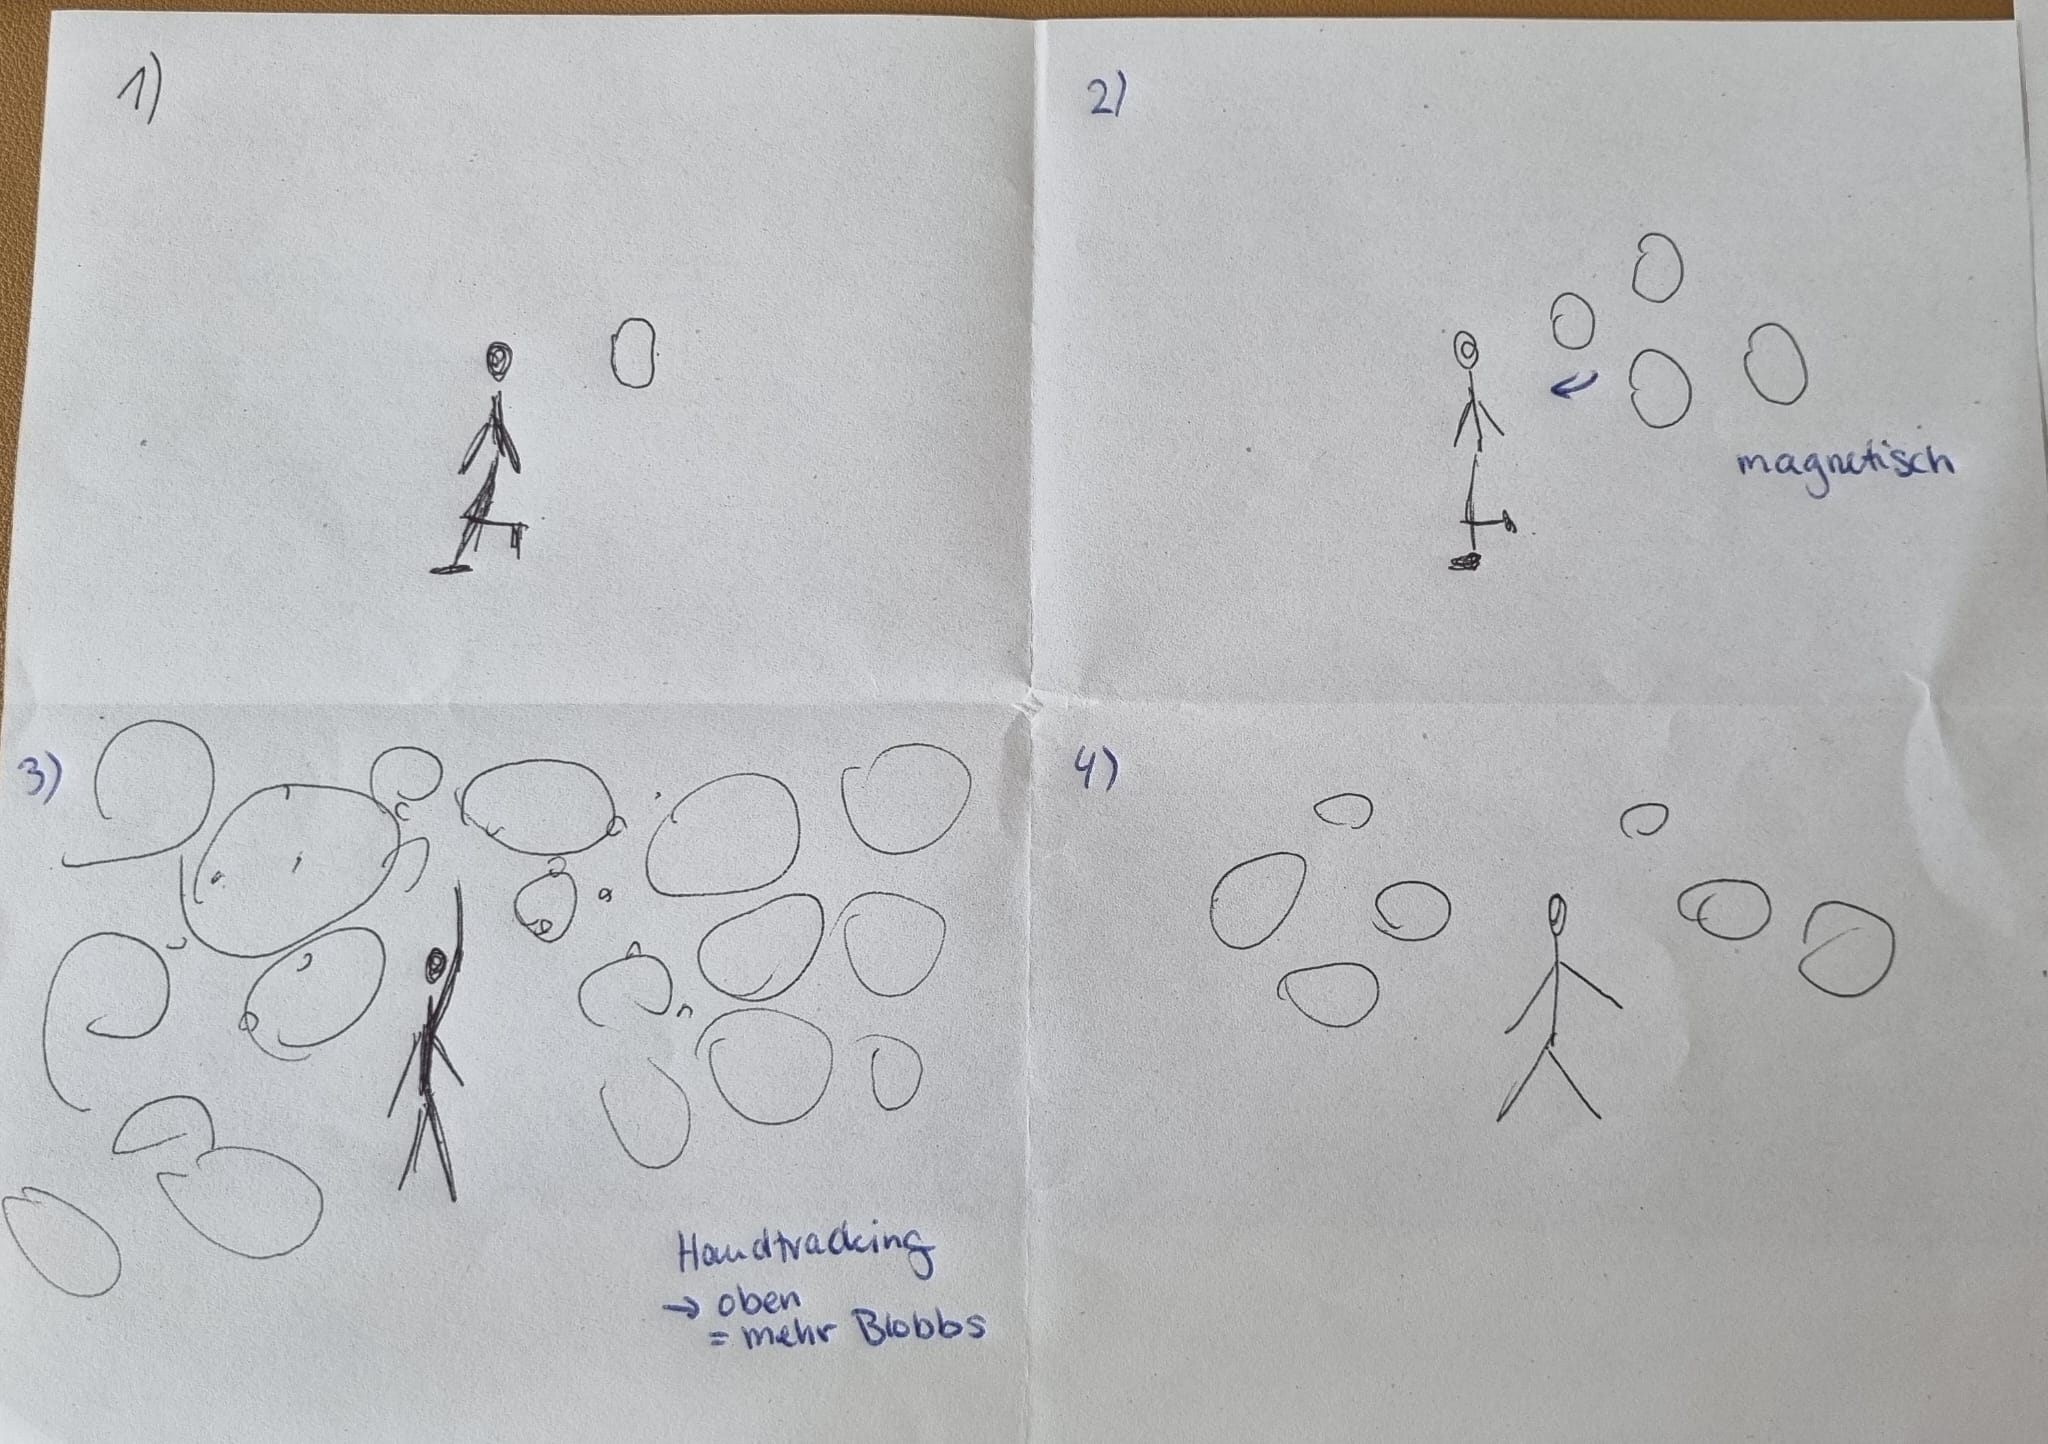
\includegraphics{images/docupictures/Sprint3_1.jpg}%
    }
    \caption{Erstes künsterlisches Konzept der Blobs: Blobs sind magnetisch anziehend/abstoßend zum Künstler}
    \label{fig:scaling_concept}
\end{figure}

\begin{figure}[htbp]
    \centering
    \adjustbox{max width=0.8\textwidth, max height=0.8\textheight, keepaspectratio}{%
        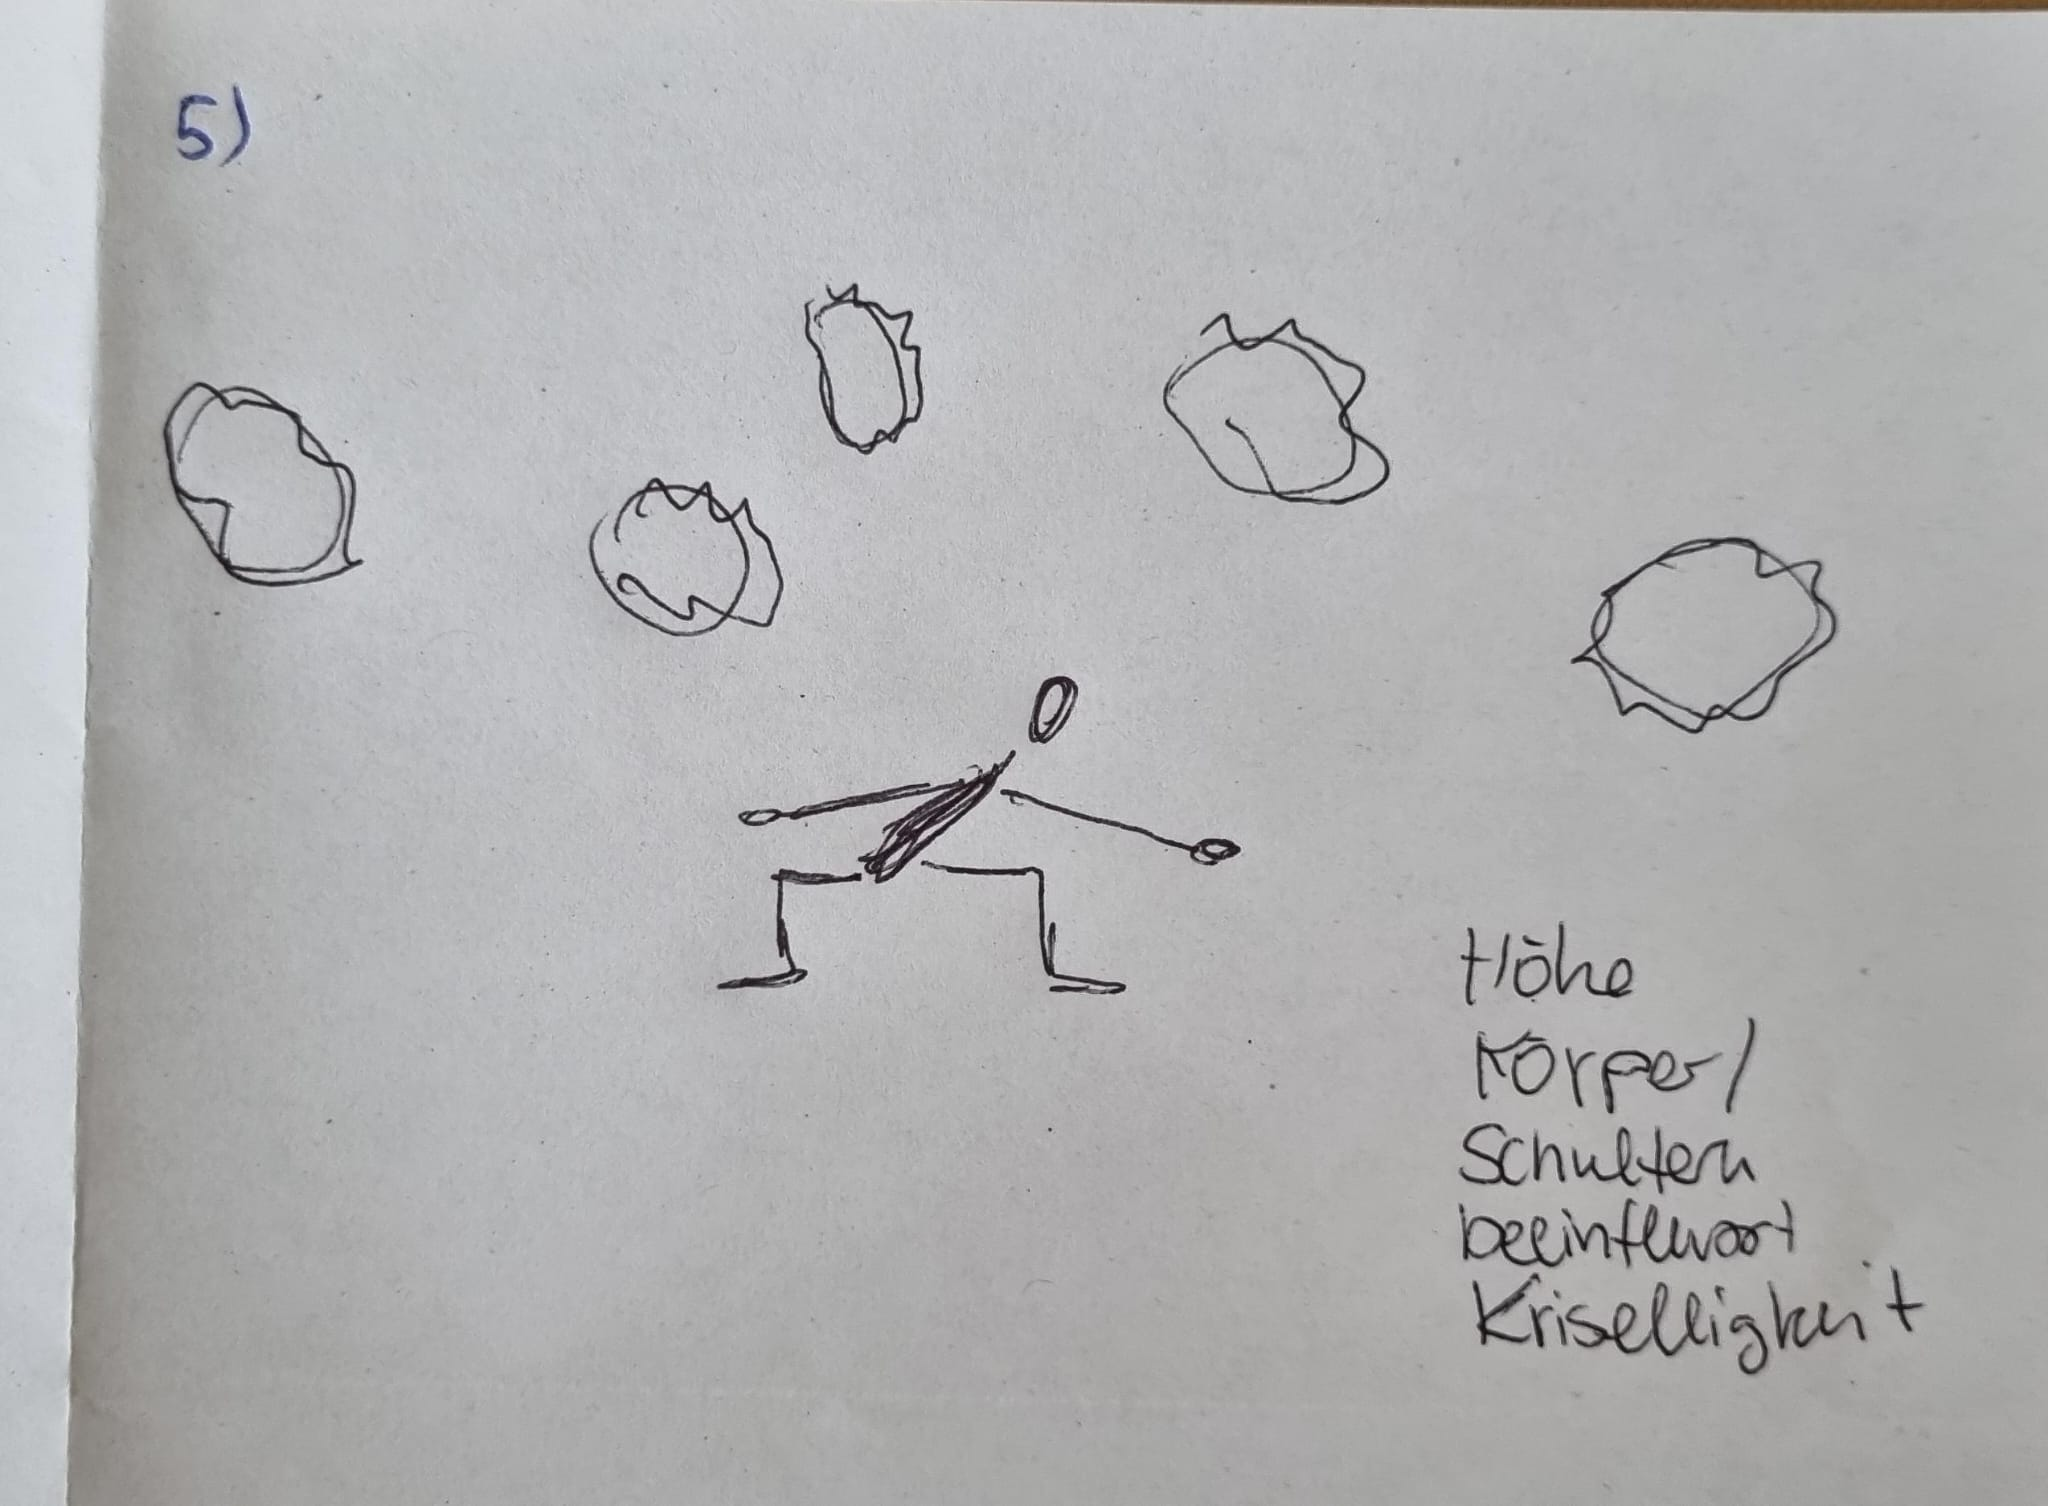
\includegraphics{images/docupictures/Sprint3_2.jpg}%
    }
    \caption{Künsterlisches Konzept, das übernommen wurde: Je nach Position des Performers werden die Blobs krisselig/blitzig oder ruhig dargestellt)}
    \label{fig:external_positioning}
\end{figure}

\begin{figure}[htbp]
    \centering
    \adjustbox{max width=0.8\textwidth, max height=0.8\textheight, keepaspectratio}{%
        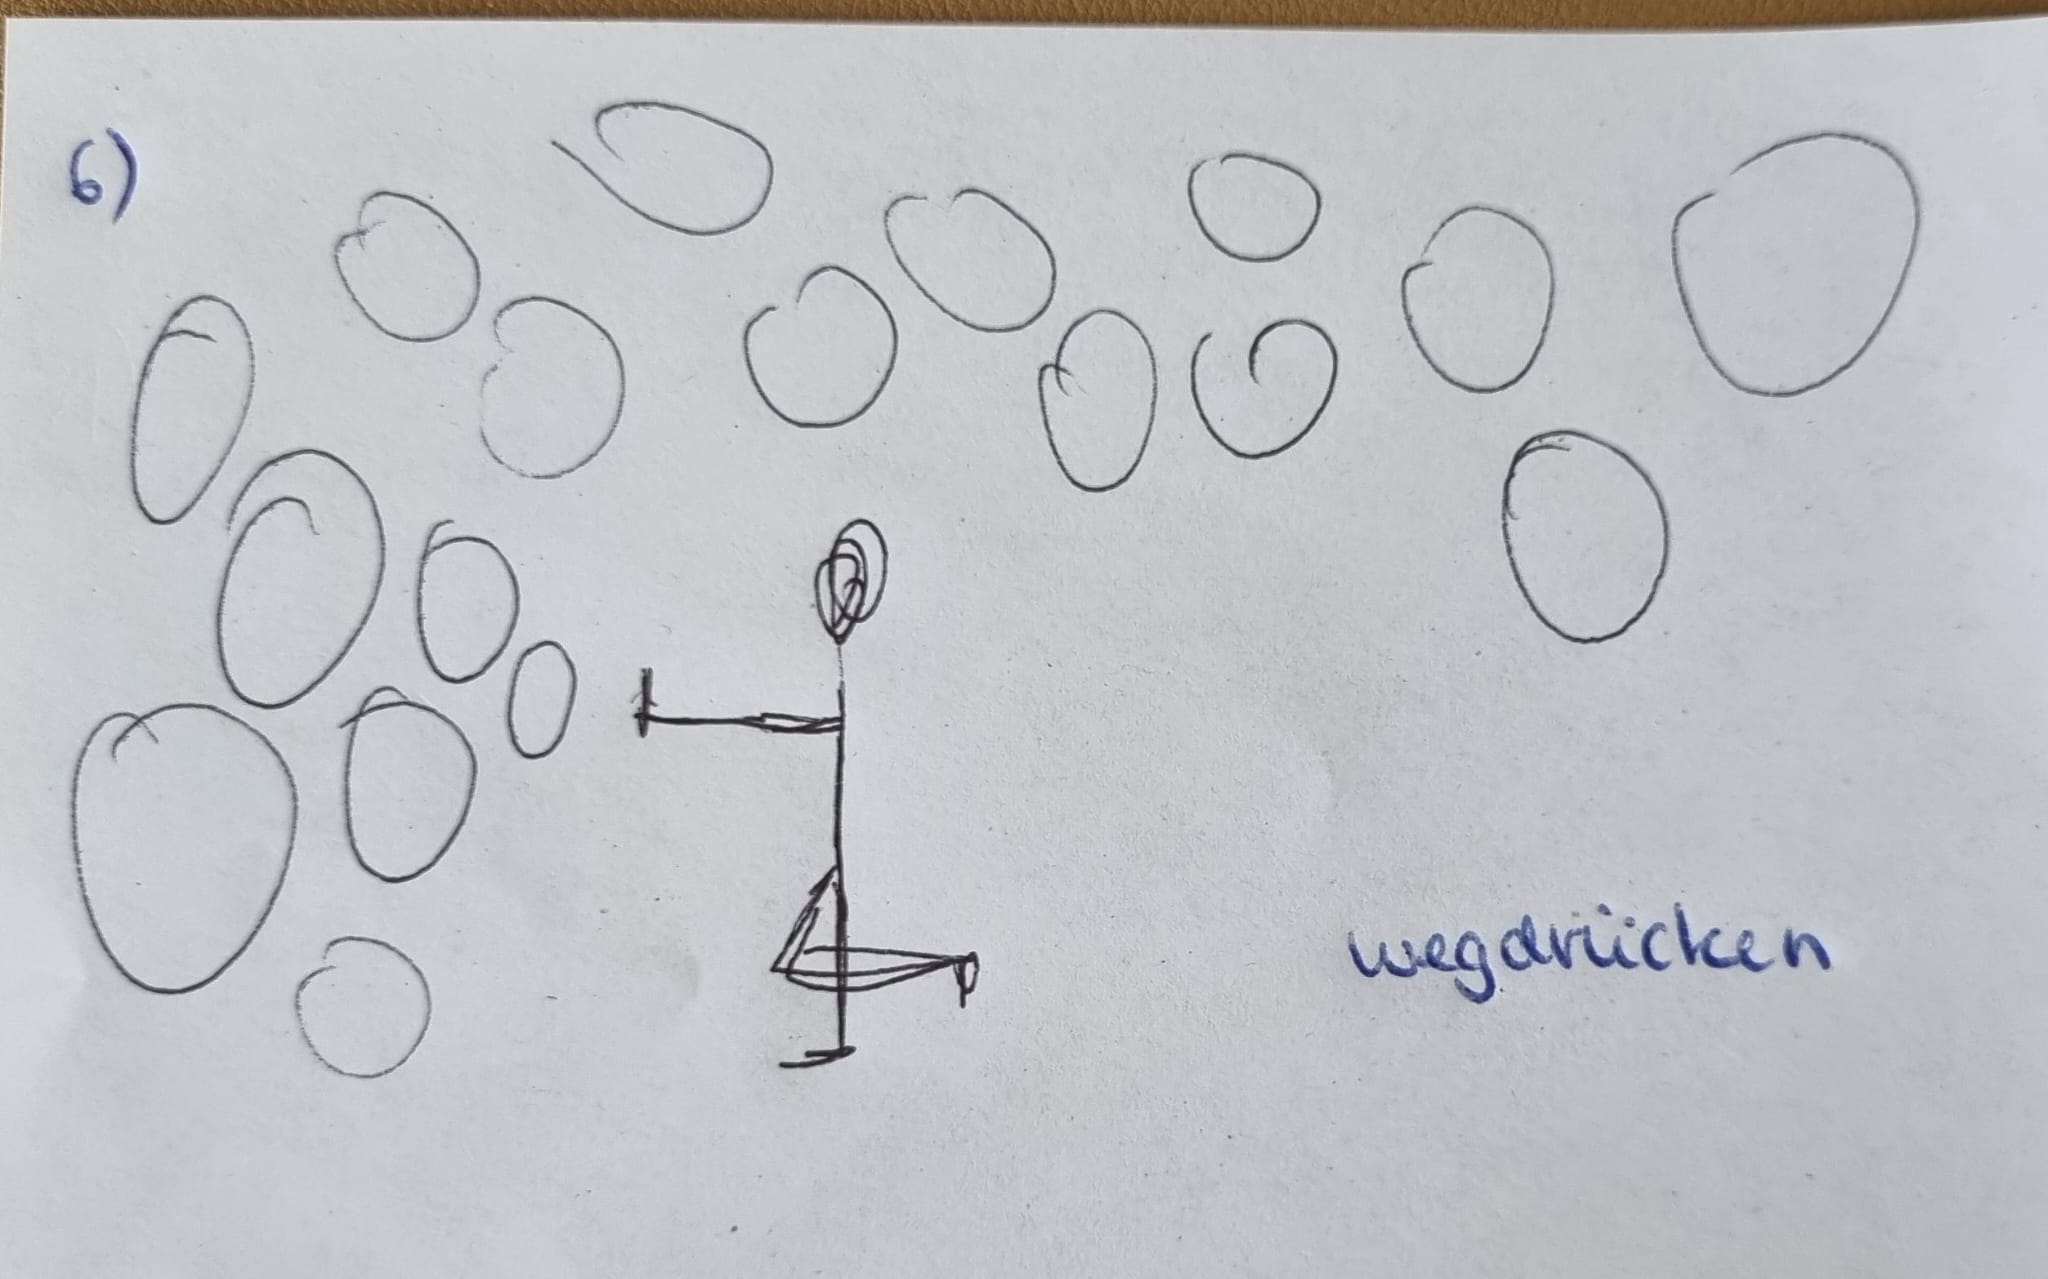
\includegraphics{images/docupictures/Sprint3_3.jpg}%
    }
    \caption{Künsterlisches Konzept, das deprecated wurde, nachdem meine Shader-Solution nicht geklappt hatte: Magnetische Interaktion: Dynamische Visual-Performer-Relation}
    \label{fig:magnetic_interaction}
\end{figure}

\begin{figure}[htbp]
    \centering
    \adjustbox{max width=0.6\textwidth, max height=0.8\textheight, keepaspectratio}{%
        
\includegraphics{images/docupictures/Sprint3_4.jpg}%
    }
    \caption{Künsterlisches Konzept, das übernommen wurde: der Performer ist in einem hellen Kreis, und bewegt sich}
    \label{fig:movement_responsive}
\end{figure}

\begin{figure}[htbp]
    \centering
    \adjustbox{max width=0.8\textwidth, max height=0.8\textheight, keepaspectratio}{%
        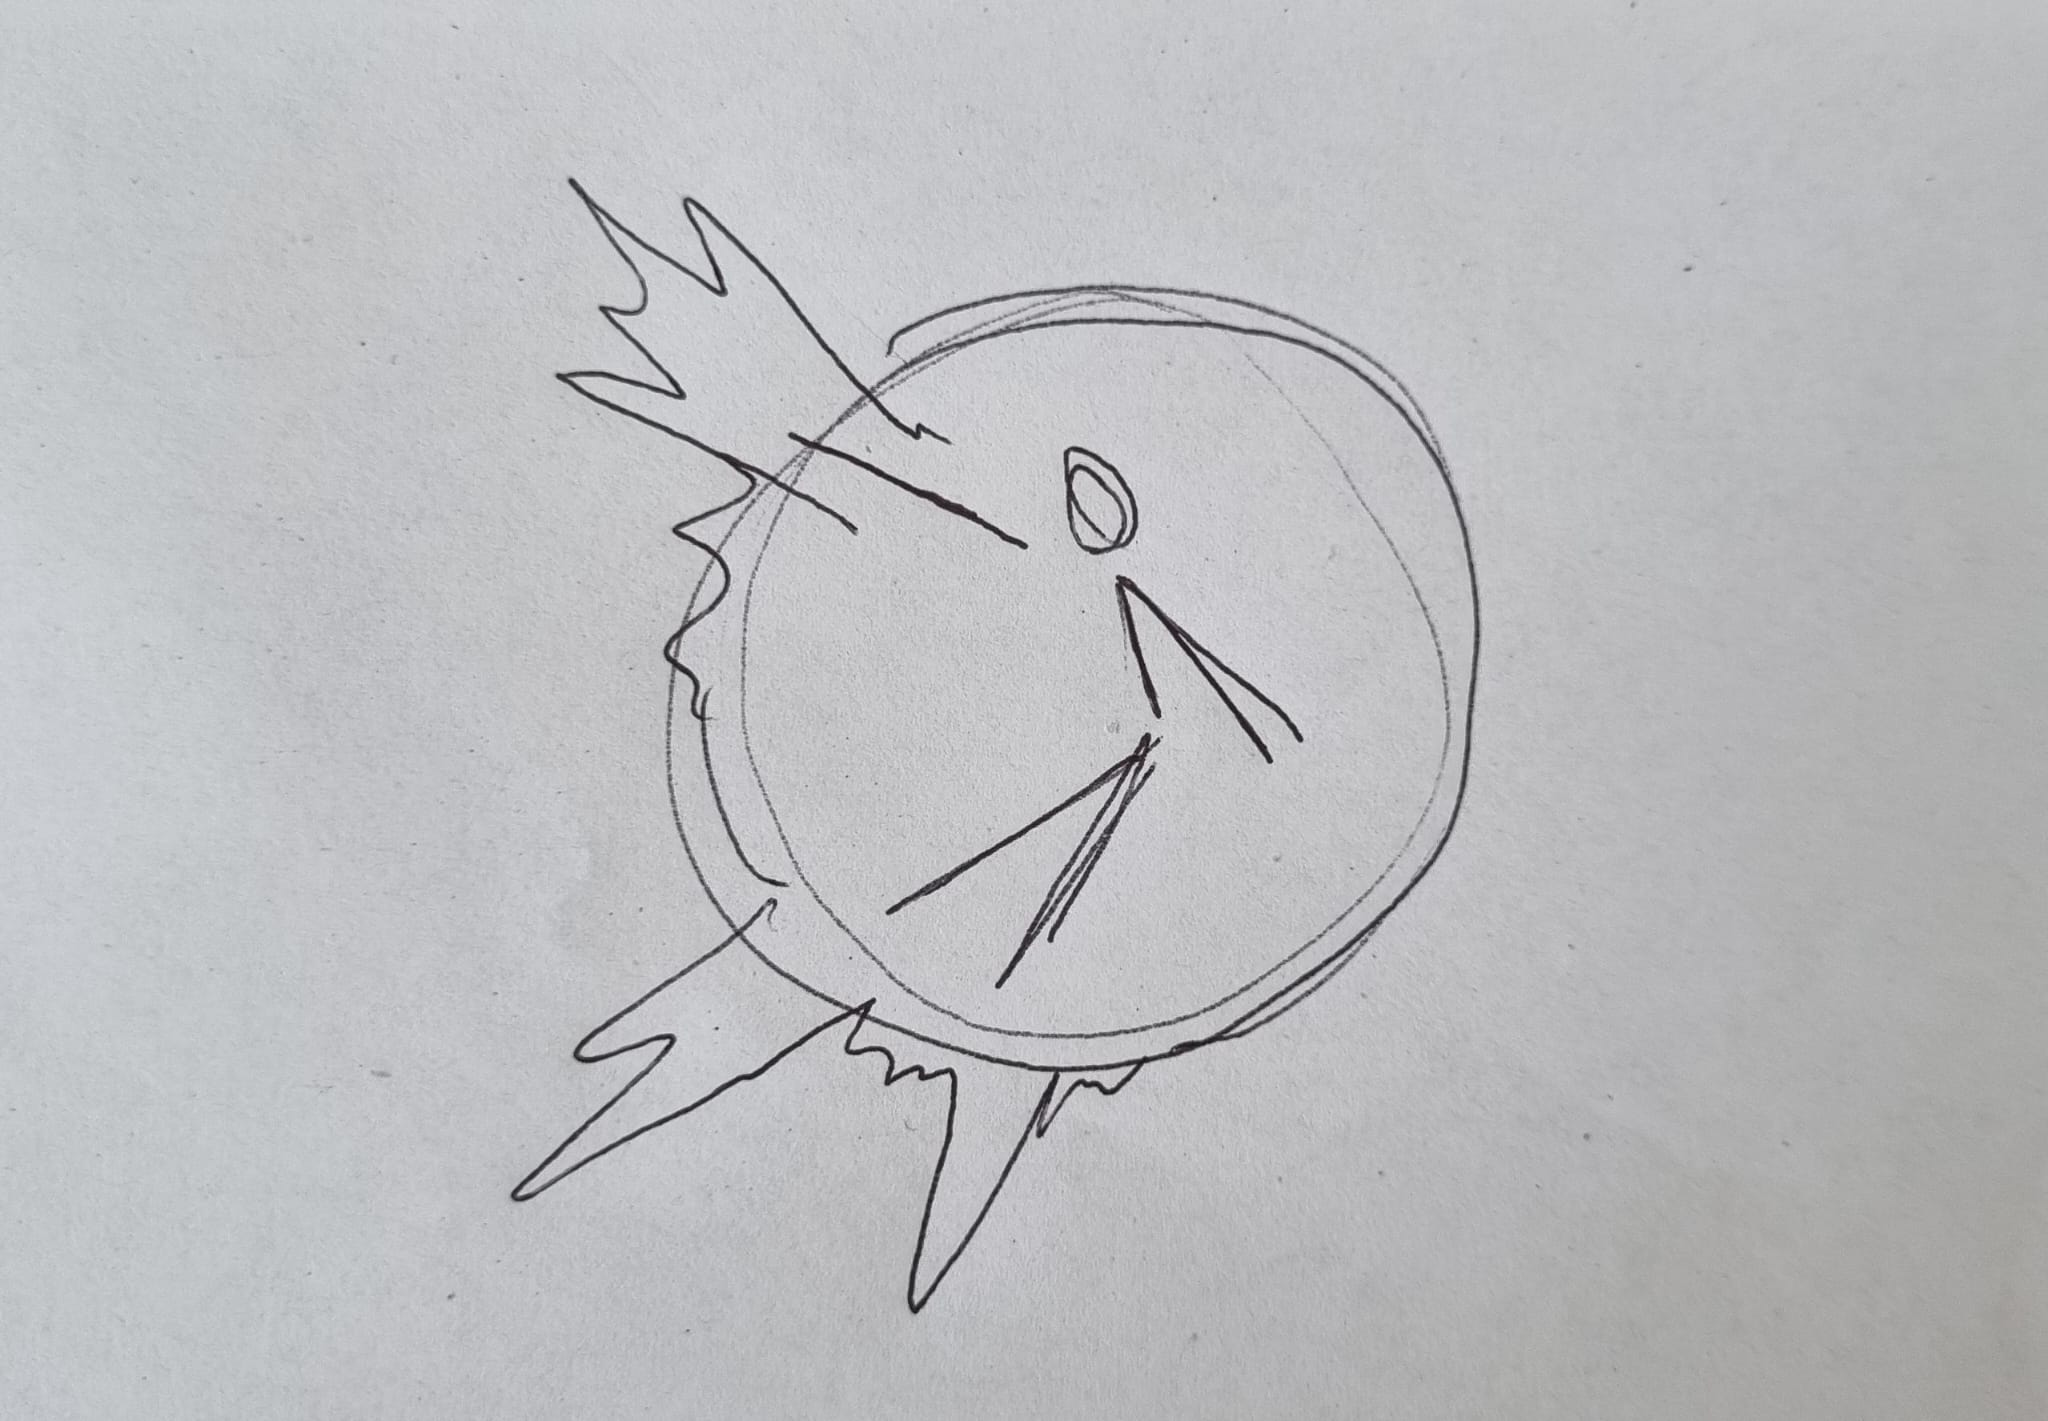
\includegraphics{images/docupictures/Sprint3_5.jpg}%
    }
    \caption{Künsterlisches Konzept, das übernommen wurde: der Performer ist in einem hellen Kreis, und die Visuals brechen interaktiv mit seinen Extremitäten-Koordinaten passend aus}
    \label{fig:composite_effects}
\end{figure}






\subsubsection{Technische Implementierungsanforderungen}

\textbf{TouchDesigner-Integration:}
\begin{itemize}
    \item Entwicklung parametrischer Visual-Generatoren
    \item Real-time Skeleton-zu-Visual-Mapping
    \item Multi-State Visual-Transition-Logik
    \item Beamer-Kalibrierung für präzise Raumprojektion
\end{itemize}

\textbf{Tracking-System-Anforderungen:}
\begin{itemize}
    \item Hochfrequente Positionsdatenausgabe (>30 FPS)
    \item Bewegungsvektor-Berechnung für Richtungserkennung
    \item Extremitäten-Tracking für spezifische Visual-Trigger
    \item Körperhaltungs-Klassifikation (stehend, hockend, gestreckt)
\end{itemize}

\textbf{Performance-Optimierung:}
\raggedright Diese Visual-Konzepte erfordern signifikante Rechenressourcen und definieren die Hardware-Mindestanforderungen für die Filmakademie-Implementation.

\subsubsection{Sprint 4 Vorbereitung}

\textbf{Deliverables für Sprint 4:}
\begin{itemize}
    \item Prototypische Umsetzung der Skalierungslogik
    \item Erste Tests der räumlichen Visual-Positionierung
    \item Bewegungsvektor-Algorithmus für dynamische Effekte
    \item Performance-Benchmarking der Visual-Pipeline
\end{itemize}